\documentclass[10pt]{article}
\usepackage[utf8]{inputenc}
\usepackage{xcolor}
%\usepackage{palatino}
\usepackage{helvet}
\renewcommand{\familydefault}{\sfdefault}
\usepackage{tikz}
\usepackage[paperwidth=20cm,paperheight=20cm,left=1cm,right=1cm,bottom=1cm,top=1cm]{geometry}
\usetikzlibrary{mindmap,backgrounds}

\pagestyle{empty}
\begin{document}
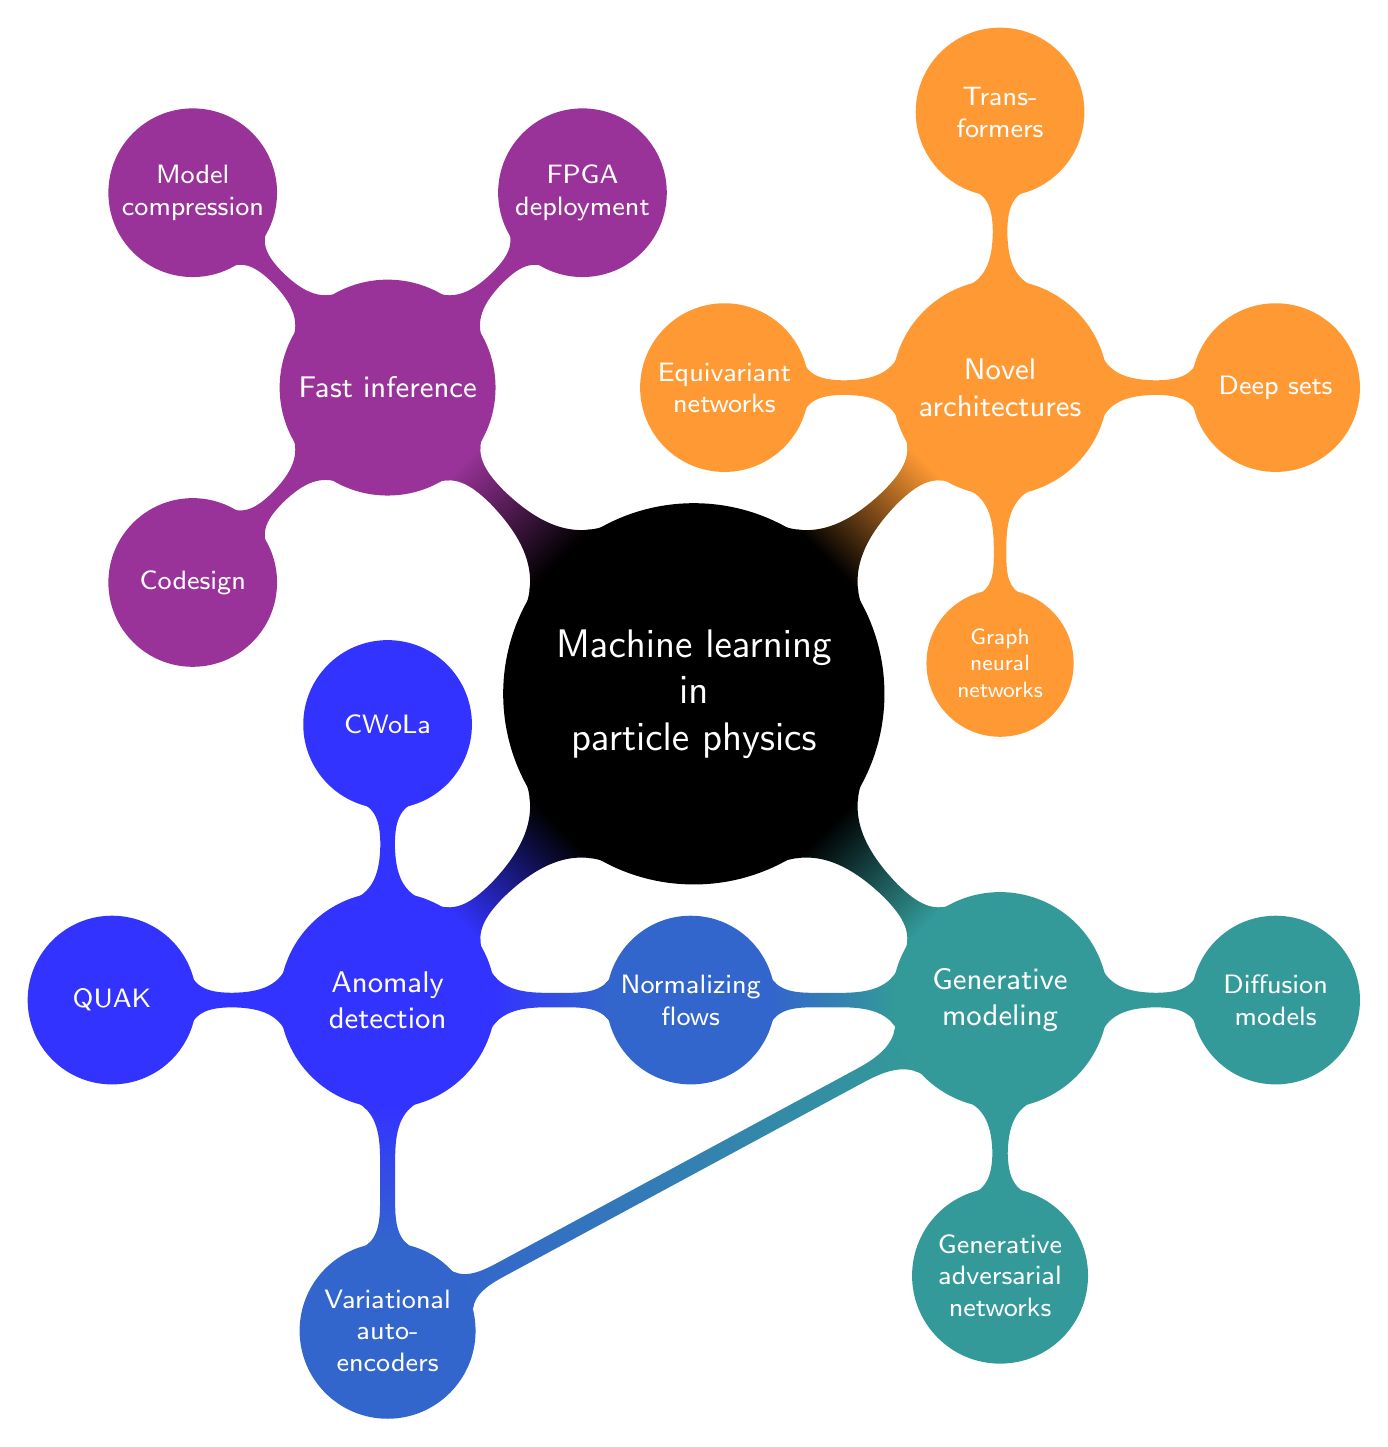
\begin{tikzpicture}[mindmap, grow cyclic, every node/.style=concept, concept color=black, text=white,
	level 1/.append style={level distance=5.5cm,sibling angle=90},
	level 2/.append style={level distance=3.5cm,sibling angle=90},]

\node [scale=1.2]{Machine learning\\in\\particle physics}
child [concept color=blue!80] { node [scale=1.2] {Anomaly detection}
	child { node [scale=1.2] {CWoLa}}
	child { node [scale=1.2] {QUAK}}
	child [concept color=blue!50!teal!80, scale=1.2] { node [scale=1.2] (vae) {Variational\\auto-\\encoders}}
	child [concept color=blue!50!teal!80, scale=1.1] { node [scale=1.2] (nf) {Normalizing flows}}
}
child [concept color=teal!80] { node [scale=1.2] (gen) {Generative modeling}
	child { node [scale=1.2] {Generative adversarial networks}}
	child { node [scale=1.2] {Diffusion models}}
}
child [concept color=orange!80] { node [scale=1.2] {Novel\\architectures}
	child { node {Graph neural networks}}
	child { node [scale=1.2] {Deep sets}}
	child { node [scale=1.2] {Trans-formers}}
	child { node [scale=1.2] {Equivariant networks}}
}
child [concept color=violet!80] { node [scale=1.2] {Fast inference}
	child { node [scale=1.2] {FPGA\\deployment}}
	child { node [scale=1.2] {Model\\compression}}
	child { node [scale=1.2] {Codesign}}
};
    \path (gen) to[circle connection bar switch color=from (teal!80) to (blue!50!teal!80)] (vae);
    \path (gen) to[circle connection bar switch color=from (teal!80) to (blue!50!teal!80)] (nf);
    
    
\end{tikzpicture}
\end{document}